\chapter{Lightweight Real-Time Feature Monitoring} \label{chap:my-work} \minitoc

Our goal is to detect data pattern shifts in an online fashion. Such shifts will be measured between a reference or normality period versus the observed reality during the streaming phase. Note that we need not to directly compare the entire window contents of the reference period with the contents of the sliding window. Doing this would mean our memory consumption grew linearly with window or reference period size. We want some sort of aggregation over the reference period that can be maintained efficiently throughout run-time and can be used to distinguish both periods of time and alert for changes. In short, we want a reference aggregation snapshot to compare with a streaming aggregation that must be updated in real-time and constant in memory usage.

\section{Approach A: Usage of outlier detection methods}
The first approach considered relied on outlier detection methods such as the ones presented in Section \ref{sec:outliers} and classified by the taxonomy in Figure \ref{fig:outlier-taxonomy}. This straightforward approach works with either subsequence or point outlier detection methods to analyze the streaming sliding window and produce data pattern shift alerts.

\subsection*{How}

Using point outlier detection methods, the main idea would be to keep track of the rate of point outliers detected. For instance, keep track of how many outliers were alerted in the past hour. The decision to alert for a data pattern shift of the system would be made when comparing this rate of point outliers detected in the past hour with a user-defined threshold $\alpha$. On the other hand, using subsequence outlier detection methods would allow us to report the whole sliding window as an outlier. 


\subsection*{Challenges}
The analyzed outlier detection algorithms in Section \ref{sec:outliers} were deemed unfit for our use-case due to one or more of the following: \textit{(a)} high memory consumption, \textit{(b)} high time complexity, \textit{(c)} "memory loss" and \textit{(d)} obfuscated insights.

In our lightweight real-time solution we need constant time complexity to process events one by one in real-time. Additionally, because our system is not mission-critical, we want a solution as lightweight as possible, which means something that grows linearly with window size is not a good fit. Therefore, most of the outlier detection methods presented become unfit for our use due to high memory consumption and time complexity. Some of the methods shown also suffer from what we call \textit{"memory loss"}: they lose track of the reference window or normality period. In other words, the algorithms are online learners, meaning they adapt to the underlying statistics of the data stream. While in some scenarios this is a much-needed feature, in our use-case it is not. How clear the alerts and insights retrieved from the methods are is also an important property. Some outlier detection methods used Machine Learning (ML) techniques to produce alerts, which makes it harder to explain to a system administrator why an alert was raised and what changed.

\subsection*{Conclusion}
We concluded that employing outlier detection methods was not the best course of action and put aside this approach.

\section{Approach B: Thresholding aggregation values}
This second approach focus on building an aggregation snapshot of the reference period to compare with streaming aggregation values and alert if the difference between both surpasses a threshold $\alpha$.

\subsection*{How}

In this approach we compute sliding window aggregations and compare the aggregations’ current state versus an initial reference, reporting a shift when the difference is substantial. For instance, consider the case where we monitor one single feature or variable \textit{x}. Assume we define the set of aggregations to compute the mean of \textit{x} and its standard deviation. Also assume we save the reference window and maintain a sliding window and the average and standard deviation aggregations for \textit{x} efficiently. As seen in Figure \ref{fig:approach2-initial-state}, the initial mean and standard deviation values for \textit{x} presented in the reference window are of 5 and 1, respectively. Later on, in \textit{Window 1}, we see the same values for the mean and standard deviation, of 5 and 1, respectively. This represents a \textit{normal} case where no alert is produced.

\begin{figure}[!htb]
    \begin{center}
      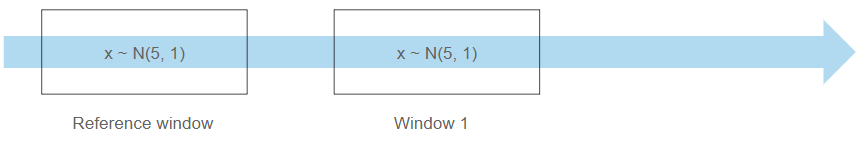
\includegraphics[scale=0.65]{figures/approach2-normality.png}
      \caption[]{Normal state for feature \textit{x} in window 1}
      \label{fig:approach2-initial-state}
    \end{center}
\end{figure}


In Figure \ref{fig:approach2-alert-state}, after further sliding steps of our sliding window, we obtain \textit{Window 2}. In \textit{Window 2}, the mean and standard deviation aggregation values change from 5 and 1 to 12 and 6, respectively. In this case, we would measure the difference between the sliding window aggregations and the reference window ones and if above a certain threshold raise an alert. For example, if we used a threshold of $\alpha$ = 6, we would raise an alert, as at least one sliding aggregation, in this case the mean, would differ of at least $\alpha$ when compared to the reference value.

\begin{figure}[!htb]
    \begin{center}
      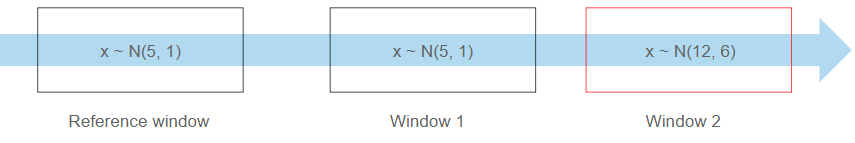
\includegraphics[scale=0.65]{figures/approach2-alert.png}
      \caption[]{Alert state for feature \textit{x} in window 2}
      \label{fig:approach2-alert-state}
    \end{center}
\end{figure}

\subsection*{Challenges}
The first issue with this approach is that generic sliding window aggregation algorithms grow linearly in space regarding window size, such as Recalculate-From-Scratch and Subtract-On-Evict presented in Section \ref{sec:back-swag-algs}, Two-Stacks has seen in Section \ref{sec:2stacks} and DABA in Section \ref{sec:daba}. Another challenge when using this approach is defining the set of aggregations to compute at feature/variable level that represent the system state well enough for comparison of reference and streaming periods and change detection. Yet another challenge would be to define the maximum deviation threshold $\alpha$  between the reference aggregation state and the streaming aggregation state to produce alerts.


Exponential Moving Averages (Section \ref{sec:emas}), Probabilistic Data Structures (Section \ref{sec:pds}) and their sliding window implementations (Section \ref{sec:sliding-pds}) can be used to solve the first issue and reduce the linear memory complexity of the system relative to sliding window size. 

However, there is no trivial solution for the second and third challenges. Defining the maximum allowed threshold between reference and sliding window aggregations does not have a straightforward solution. Furthermore, defining the set of aggregations to use is also a big challenge. To illustrate, consider both time-series show in Figure \ref{fig:approach2-timeseries}.
 
\begin{figure}[!htb]
    \begin{center}
      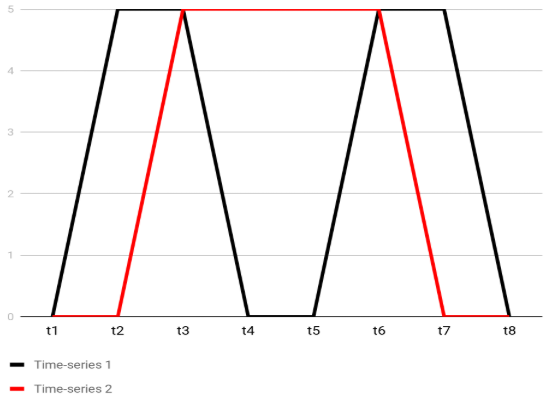
\includegraphics[scale=0.65]{figures/approach2-timeseries.png}
      \caption[]{Alert state for feature \textit{x} in window 2}
      \label{fig:approach2-timeseries}
    \end{center}
\end{figure}


Both time-series 1 and 2 have the same maximum, minimum, mean and standard deviation values for the time-based window between \textit{t\textsubscript{1}} and \textit{t\textsubscript{8}}. Hence, if our set of aggregations chosen were the maximum, minimum, mean and standard deviation, we would not differentiate between these two clearly different time-series.

\subsection*{Conclusion}
This approach requires efficient sliding window aggregation state maintenance, which can be done using sliding window probabilistic data structures and/or exponential moving averages. However, defining the set of aggregations to use and the deviation threshold itself ultimately led us to discard this approach.


\section{Proposed method: Numerical Feature Monitoring}
%what we want (reiterate)
%A reference aggregation snapshot to compare with a streaming aggregation that must be kept in real-time and constant in memory usage

%- introduce method as two-phased method (batch and streaming)

% only for numerical features for now

\subsection{Stream monitoring goals}
%- what is our goal in the streaming phase?
           % - alert when streaming fields/features/variables' distribution changes considerably
          %  - need to choose an aggregation that allows us to know the distribution of variables -> histogram for each feature
               % - lightweight -> approximated EMA-based histogram (recall EMAs background), each bin count is an EMA-count aggregation
               % - describe an EMA approximated histogram and how it discounts old events, the simulated window size, ...
           % - we can compute an exact histogram over the reference period because it is done in batch, where resources like RAM or time are not heavily constrained in constrast to streaming systems
           % - given 2 histograms (ref hist and stream hist) we can apply distance metrics (such as a JSD)
             %   - worth mentioning other metrics can be used (Wasserstein distance, Kolmogorov–Smirnov, ...)
         %   - but how to threshold this "distance" value? ----> we need to know the distribution of "distance" values
             %   - how is this accomplished
             %   - agressive sampling within ref period of smaller periods (equal in size to the stream simulated window)
              %  - give a practical use-case where it makes a diference:
                 %   - left-skewed distro vs right-skewed distro ---> threshold is very different (95 or 99 percentile for example)

\subsection{Batch analysis phase}

%- batch phase: build reference exact histogram and distribution of distance values
          %  1. compute ref histogram (for each feature)
                %- equal heights/counts per bin, different size bins ---> better adjusted to wildly varying distributions
         %   2. make samples of length equal to streaming window size, build histograms for each using bins from reference histogram to make later accurate comparisons between ref hist and sample hist
             %   - why multiple sample histograms?
                   % encode distributions over smaller time periods since there may be pattern changes within the large reference period
             %   - why an approximated histogram for the samples as well despite being done in batch?
                 %   mimic the streaming approximated histogram and the test that will be performed:
                     %   - batch: sample app. histogram vs ref hist
                    %    - stream: streaming app. histogram vs ref hist
         %   3. compute the distance between each sample's histogram and the reference one (for each feature)
          %  4. we now have a list of distance values, and know their expected distribution (for each feature)
              %  - this is important since a test value obtained measuring the distance between the reference period and other window
                %can be compared to this distribution (again probably give the left and right skewed example)

          %  By the end of the batch phase we have:
               % for each feature:
                    %reference histogram (for later comparison with streaming histogram)
                    %list/histogram of distance values
                    %last sample's histogram ---> used as burn-in period for target histogram
                    
\subsection{Streaming phase}

%- online phase:
          %  for each feature:
            %    1. initialize the streaming histogram as the last sample's histogram from the batch phase (burn-in period)
            
         %   for each event:
               % for each field/feature:
                  %  1. update the feature's streaming histogram (recall the update method)
                  %  2. compute the distance between the reference histogram and the target histogram
                   % 3. test the percentile the distance value fits according to the feature's distances list and alert if above a certain percentile (say the 99th)

           % introduce the multiple testing correction problem:
              %  "the more inferences are made, the more likely erroneous inferences are to occur"
             %   we are making multiple hypothesis testing when computing a distance and checking the percentile for each feature

                %introduce the Holm-Bonferroni multiple test correction method
            
            %So in reality we have:

          %  for each event:
               % for each field/feature:
                 %   1. update the feature's streaming histogram (recall the update method)
                  %  2. compute the distance between the reference histogram and the target histogram
                  %  3. apply holm-bonferroni for all feature's distances:
                     %   - each percentile will be a p-value
                    %    - order features by p-value
                    %    - check if p-value > FWER / (m + 1 - k)
                          %  if so then feature is divergent
                          
\subsection{Summary}